\PassOptionsToPackage{unicode=true}{hyperref} % options for packages loaded elsewhere
\PassOptionsToPackage{hyphens}{url}
%
\documentclass[]{article}
\usepackage{lmodern}
\usepackage{amssymb,amsmath}
\usepackage{ifxetex,ifluatex}
\usepackage{fixltx2e} % provides \textsubscript
\ifnum 0\ifxetex 1\fi\ifluatex 1\fi=0 % if pdftex
  \usepackage[T1]{fontenc}
  \usepackage[utf8]{inputenc}
  \usepackage{textcomp} % provides euro and other symbols
\else % if luatex or xelatex
  \usepackage{unicode-math}
  \defaultfontfeatures{Ligatures=TeX,Scale=MatchLowercase}
\fi
% use upquote if available, for straight quotes in verbatim environments
\IfFileExists{upquote.sty}{\usepackage{upquote}}{}
% use microtype if available
\IfFileExists{microtype.sty}{%
\usepackage[]{microtype}
\UseMicrotypeSet[protrusion]{basicmath} % disable protrusion for tt fonts
}{}
\IfFileExists{parskip.sty}{%
\usepackage{parskip}
}{% else
\setlength{\parindent}{0pt}
\setlength{\parskip}{6pt plus 2pt minus 1pt}
}
\usepackage{hyperref}
\hypersetup{
            pdftitle={Description des données d'usage de la base ESTAMP},
            pdfborder={0 0 0},
            breaklinks=true}
\urlstyle{same}  % don't use monospace font for urls
\usepackage[margin=1in]{geometry}
\usepackage{longtable,booktabs}
% Fix footnotes in tables (requires footnote package)
\IfFileExists{footnote.sty}{\usepackage{footnote}\makesavenoteenv{longtable}}{}
\usepackage{graphicx,grffile}
\makeatletter
\def\maxwidth{\ifdim\Gin@nat@width>\linewidth\linewidth\else\Gin@nat@width\fi}
\def\maxheight{\ifdim\Gin@nat@height>\textheight\textheight\else\Gin@nat@height\fi}
\makeatother
% Scale images if necessary, so that they will not overflow the page
% margins by default, and it is still possible to overwrite the defaults
% using explicit options in \includegraphics[width, height, ...]{}
\setkeys{Gin}{width=\maxwidth,height=\maxheight,keepaspectratio}
\setlength{\emergencystretch}{3em}  % prevent overfull lines
\providecommand{\tightlist}{%
  \setlength{\itemsep}{0pt}\setlength{\parskip}{0pt}}
\setcounter{secnumdepth}{5}
% Redefines (sub)paragraphs to behave more like sections
\ifx\paragraph\undefined\else
\let\oldparagraph\paragraph
\renewcommand{\paragraph}[1]{\oldparagraph{#1}\mbox{}}
\fi
\ifx\subparagraph\undefined\else
\let\oldsubparagraph\subparagraph
\renewcommand{\subparagraph}[1]{\oldsubparagraph{#1}\mbox{}}
\fi

% set default figure placement to htbp
\makeatletter
\def\fps@figure{htbp}
\makeatother

\usepackage{etoolbox}
\makeatletter
\providecommand{\subtitle}[1]{% add subtitle to \maketitle
  \apptocmd{\@title}{\par {\large #1 \par}}{}{}
}
\makeatother

\title{Description des données \emph{d'usage} de la base ESTAMP}
\providecommand{\subtitle}[1]{}
\subtitle{LifePAP}
\author{}
\date{\vspace{-2.5em}}

\begin{document}
\maketitle

{
\setcounter{tocdepth}{5}
\tableofcontents
}
\textbf{Contexte}

La réalisation des données d'usage nécessite au préalable de décrire les
données présentes dans la base ESTAMP. Cette description permettra de
mettre en avant les points forts et les points faibles permettant ainsi
d'élaborer d'éventuelles solutions pour améliorer la
robustesse{[}\^{}2{]} de la base.

Les données ont été extraites le 28-04-2020 via le site web
(\url{https://estamp.afbiodiversite.fr/}).

L'extraction est composée de 7 fichiers :

\begin{verbatim}
enquete_connaissance_pecheur.csv 
enquete_detail.csv 
enquete_peche_jour.csv 
enquete_pratique_peche.csv 
enquete_preparation_peche.csv 
ficheterrain.csv 
ProtocolesEnquetesPaP.pdf
\end{verbatim}

\hypertarget{description-des-donnuxe9es-extraites}{%
\subsubsection{\texorpdfstring{\textbf{1 Description des données
extraites}}{1 Description des données extraites}}\label{description-des-donnuxe9es-extraites}}

Le jeu de données est composé de 5997 lignes (= observations) et 144
colonnes (= variables)

\begin{longtable}[]{@{}llrrl@{}}
\toprule
Variable & Class & Nombre\_Elements & Nombre\_NA &
Exemples\tabularnewline
\midrule
\endhead
libelle\_sortie & character & 5997 & 0 & Le Veillon\_22/09/2016\_Justine
VALLEE\_S00006\tabularnewline
Libellé Sortie.x & character & 5997 & 0 & Le
Veillon\_22/09/2016\_Justine VALLEE\_S00006\tabularnewline
Code Enquète.x & character & 0 & 5997 & :\tabularnewline
Observateurs & character & 81 & 162 & Justine VALLEE\tabularnewline
Num Enquéte & character & 5997 & 0 & S00006\tabularnewline
Heure Début & hms & 0 & 5997 & :\tabularnewline
Enquete Hors Panier & character & 1 & 0 & Non renseigné :
5997\tabularnewline
Panier Complet & character & 1 & 0 & Non renseigné : 5997\tabularnewline
Pecheur Sensibilisé & character & 1 & 0 & Non renseigné :
5997\tabularnewline
Pecheur enqueté & character & 1 & 0 & Non renseigné :
5997\tabularnewline
Constitution Groupe & character & 0 & 5997 & :\tabularnewline
Nb adultes & integer & 0 & 5997 & :\tabularnewline
Nb enfants & integer & 0 & 5997 & :\tabularnewline
Nb tous petits & integer & 0 & 5997 & :\tabularnewline
Nb pecheurs groupe & integer & 30 & 173 & 2\tabularnewline
Nb Pecheurs Sensibilises & integer & 87 & 97 & 2\tabularnewline
Nb Reglettes & integer & 78 & 105 & 1\tabularnewline
Nb Depliants & integer & 8 & 3287 & 0 : 2096 - 1 : 497 - 2 : 97 - 3 : 9
- 4 : 6 - 5 : 2 - 7 : 2 - 12 : 1\tabularnewline
Observations & character & 1 & 5973 & Pêche dans concession :
24\tabularnewline
Annuaire de marée & character & 0 & 5997 & :\tabularnewline
Etat Sanitaire & character & 0 & 5997 & :\tabularnewline
Source d'information & character & 0 & 5997 & :\tabularnewline
Equipé Téléphone portable & character & 0 & 5997 & :\tabularnewline
Connaissance Numéro Secours & character & 0 & 5997 & :\tabularnewline
Numéro Secours & character & 0 & 5997 & :\tabularnewline
Critéres choix site & character & 0 & 5997 & :\tabularnewline
ID fiche & character & 5997 & 0 & 316971\tabularnewline
type de suivi & character & 1 & 0 & Suivi des enquêtes pêcheurs à pied :
5997\tabularnewline
date sortie & POSIXct & 243 & 0 & 2016-09-22\tabularnewline
heure début & hms & 0 & 5997 & :\tabularnewline
heure fin & hms & 0 & 5997 & :\tabularnewline
coefficient marée & integer & 62 & 2 & 70\tabularnewline
heure marée basse & hms & 237 & 72 & 15:37:00\tabularnewline
hauteur basse mer & numeric & 0 & 5997 & :\tabularnewline
période & character & 3 & 1856 & Semaine : 941 - Vacances : 2896 -
Week-end ou Jour Férié : 304\tabularnewline
libellé campagne & character & 0 & 5997 & :\tabularnewline
référent sortie & character & 81 & 162 & Justine VALLEE\tabularnewline
équipe terrain & character & 81 & 162 & Justine VALLEE\tabularnewline
territoire & character & 2 & 0 & Estuaire de la Gironde et Mer des
Pertuis : 4463 - Golfe Normand Breton : 1534\tabularnewline
code site & character & 61 & 0 & EGMP\_003\tabularnewline
site & character & 61 & 0 & Le Veillon\tabularnewline
zone & character & 0 & 5997 & :\tabularnewline
type protocole & character & 1 & 0 & Enquête sensibilisation :
5997\tabularnewline
version protocole & character & 1 & 0 & LifePAP : 5997\tabularnewline
auteur saisie & character & 1 & 0 & SYSTEME : 5997\tabularnewline
organisme suivi & character & 2 & 0 & Mission d'étude du golfe
normand-breton : 1534 - Parc naturel marin de l'estuaire de la Gironde
et de la mer des Pertuis : 4463\tabularnewline
couverture nuageuse & character & 4 & 3597 & 0-25\% (Peu ou pas nuageux)
: 326 - 25-75\% (Nuageux) : 1324 - 75-100\% (Très nuageux) : 617 -
Brouillard : 133\tabularnewline
précipitations & character & 5 & 2052 & Averses violentes ou orageuses -
Grêles ou neige : 46 - Pas de précipitation : 3778 - Pluie continue : 29
- Pluie fine : 80 - Pluies éparses : 12\tabularnewline
pression atmosphérique & numeric & 0 & 5997 & :\tabularnewline
température & numeric & 55 & 2259 & 20\tabularnewline
force du vent & character & 6 & 2370 & 1-Très légère brise-1 à 5
km/h-Mer ridée : 84 - 2-Lègère brise-6 à 11 km/h-Vaguelettes : 480 -
3-Petite brise-12 à 19 km/h-Très petites vagues. Déferlement. : 1800 -
4-Jolie brise-20 à 28 km/h-Petites vagues. Moutons. : 991 - 5-Bonne
brise-29 à 38 km/h-Vagues modérées. : 269 - 6-Vent frais-39 à 49
km/h-Crêtes d'écume blanches. : 3\tabularnewline
force du vent en rafale & character & 0 & 5997 & :\tabularnewline
direction du vent & character & 8 & 2394 & Est : 199 - Nord : 73 -
Nord-Est : 509 - Nord-Ouest : 1311 - Ouest : 603 - Sud : 196 - Sud-Est :
215 - Sud-Ouest : 497\tabularnewline
état de la mer & character & 4 & 4306 & 0-calme-0 m : 152 - 1-ridée-0 à
0,1 m : 778 - 2-belle-0,1 à 0,5 m : 487 - 3-peu agitée-0,5 à 1,25 m :
274\tabularnewline
commentaires & character & 1 & 0 & Reprise de données
Enquete\tabularnewline
: 5997 & & & &\tabularnewline
Milieu(x) & character & 5 & 5760 & Champs de blocs : 30 - Champs de
blocs \textbar{} Massifs d'hermelles : 73 - Concessions de culture : 100
- Herbiers zostères : 17 - Massifs d'hermelles : 17\tabularnewline
Espéces & character & 37 & 4739 & Palourdes croisées \textbar{}
Praire\tabularnewline
Outils ou techniques & character & 0 & 5997 & :\tabularnewline
Conformité outil(s) & character & 0 & 5997 & :\tabularnewline
Estimation Reglement & character & 0 & 5997 & :\tabularnewline
Connaissance Reglement & character & 0 & 5997 & :\tabularnewline
Premiere Peche & character & 0 & 5997 & :\tabularnewline
Annee Premiere Peche & integer & 0 & 5997 & :\tabularnewline
Peche Chaque Annee & character & 0 & 5997 & :\tabularnewline
Frequence Declaree Peche & numeric & 0 & 5997 & :\tabularnewline
Mois de peche & character & 0 & 5997 & :\tabularnewline
Nb Peches Annuelles & numeric & 0 & 5997 & :\tabularnewline
Péche du jour & character & 0 & 5997 & :\tabularnewline
Frequence Indiquee & character & 0 & 5997 & :\tabularnewline
Espéces prélevées & character & 0 & 5997 & :\tabularnewline
Prélèvement annuel poids & character & 0 & 5997 & :\tabularnewline
Prélèvement annuel nombre & character & 0 & 5997 & :\tabularnewline
Choix des marées & character & 0 & 5997 & :\tabularnewline
Coefficient Maree Mini & integer & 0 & 5997 & :\tabularnewline
Coefficient Maree NSP & character & 0 & 5997 & :\tabularnewline
Autre Sites fréquentés & character & 0 & 5997 & :\tabularnewline
Départements & character & 0 & 5997 & :\tabularnewline
Nom sites & character & 0 & 5997 & :\tabularnewline
Motivation(s) & character & 0 & 5997 & :\tabularnewline
Autres types de peche & character & 0 & 5997 & :\tabularnewline
Heure début récolte & hms & 0 & 5997 & :\tabularnewline
Temps passé récolte & numeric & 0 & 5997 & :\tabularnewline
Temps total Peche & numeric & 0 & 5997 & :\tabularnewline
Nb pêcheurs récolte & numeric & 0 & 5997 & :\tabularnewline
Panier vide & character & 3 & 0 & Non : 2684 - Non renseigné : 3311 -
Oui : 2\tabularnewline
Conformité maille & character & 3 & 3169 & Conformité \textless{} 50\% :
436 - Conformité \textgreater{} 90\% : 1421 - Conformité entre 50\% et
90\% : 971\tabularnewline
Conformité quantité & character & 0 & 5997 & :\tabularnewline
Tri du panier & character & 0 & 5997 & :\tabularnewline
Espece & character & 0 & 5997 & :\tabularnewline
Poids récolte & numeric & 0 & 5997 & :\tabularnewline
Nb individus & numeric & 0 & 5997 & :\tabularnewline
Volume récolté & numeric & 0 & 5997 & :\tabularnewline
Type évaluation & character & 0 & 5997 & :\tabularnewline
Poids maille & character & 0 & 5997 & :\tabularnewline
Nb maille & numeric & 0 & 5997 & :\tabularnewline
Volume maille & numeric & 0 & 5997 & :\tabularnewline
Type évaluation maille & character & 0 & 5997 & :\tabularnewline
Taille échantillon & numeric & 0 & 5997 & :\tabularnewline
Commune résidence & character & 0 & 5997 & :\tabularnewline
Département & character & 0 & 5997 & :\tabularnewline
Pays & character & 0 & 5997 & :\tabularnewline
De passage & character & 1 & 0 & en séjour sur une commune :
5997\tabularnewline
Commune séjour & character & 0 & 5997 & :\tabularnewline
Durée séjour & integer & 0 & 5997 & :\tabularnewline
Hebergement & character & 0 & 5997 & :\tabularnewline
Premier Séjour & character & 0 & 5997 & :\tabularnewline
Fréquence Visites & numeric & 0 & 5997 & :\tabularnewline
Influence Destination & character & 0 & 5997 & :\tabularnewline
Influence Date & character & 0 & 5997 & :\tabularnewline
Sexe - Pécheur & character & 0 & 5997 & :\tabularnewline
Annee Naissance - Pécheur & integer & 0 & 5997 & :\tabularnewline
CSP - Pécheur & character & 0 & 5997 & :\tabularnewline
Sexe - Autre membre & character & 0 & 5997 & :\tabularnewline
Annee Naissance - Autre membre & integer & 0 & 5997 & :\tabularnewline
CSP - Autre membre & character & 0 & 5997 & :\tabularnewline
Tri récolte & character & 0 & 5997 & :\tabularnewline
Accueil & character & 1 & 5877 & Refus : 120\tabularnewline
Sensibilisation & character & 0 & 5997 & :\tabularnewline
Remarques pécheur & character & 4 & 2976 & Conflits d'usage : 87 - Etat
sanitaire : 113 - Réglementation : 1991 - Ressource/Environnement :
830\tabularnewline
Précisions remarques & character & 1016 & 4574 & Intéressé par le
panneau mis en place\tabularnewline
Libellé Sortie & character & 5997 & 0 & Le Veillon\_22/09/2016\_Justine
VALLEE\_S00006\tabularnewline
Code Enquète & character & 0 & 5997 & :\tabularnewline
Membre Association & character & 0 & 5997 & :\tabularnewline
Nom Association & character & 0 & 5997 & :\tabularnewline
Espéce maille & character & 0 & 5997 & :\tabularnewline
declaration Connaissance & character & 0 & 5997 & :\tabularnewline
Taille déclarée & integer & 0 & 5997 & :\tabularnewline
connaissance réglementation & character & 0 & 5997 & :\tabularnewline
Utilisation outil & character & 3 & 512 & Non : 4451 - Oui : 894 - Oui
mais pas aujourd'hui : 140\tabularnewline
Source outil & character & 7 & 5047 & Anatomique (phalange, largeur de
paume, pouce…) : 18 - Artisanal : 371 - Autre type de réglette : 83 -
Commerce : 19 - Pied à coulisse FNPPSF : 43 - Réglette à visuels (Type
Vivarmor) : 35 - Reglette LIFE : 381\tabularnewline
Type d'outil & character & 0 & 5997 & :\tabularnewline
Outil Conforme & character & 2 & 3973 & Non : 1472 - Oui :
552\tabularnewline
Espèce quantité & character & 0 & 5997 & :\tabularnewline
Connaissance quota & character & 0 & 5997 & :\tabularnewline
Quantité déclarée & integer & 0 & 5997 & :\tabularnewline
Unite & character & 0 & 5997 & :\tabularnewline
Reglementation Quantité & character & 0 & 5997 & :\tabularnewline
Espèce période & character & 0 & 5997 & :\tabularnewline
Connaissance Période & character & 0 & 5997 & :\tabularnewline
Périodes Déclarées & character & 0 & 5997 & :\tabularnewline
Connaissance Règlementation Période & character & 0 & 5997 &
:\tabularnewline
Informé Législation & character & 0 & 5997 & :\tabularnewline
Source information législation & character & 0 & 5997 & :\tabularnewline
Conseils consommation & character & 0 & 5997 & :\tabularnewline
\bottomrule
\end{longtable}

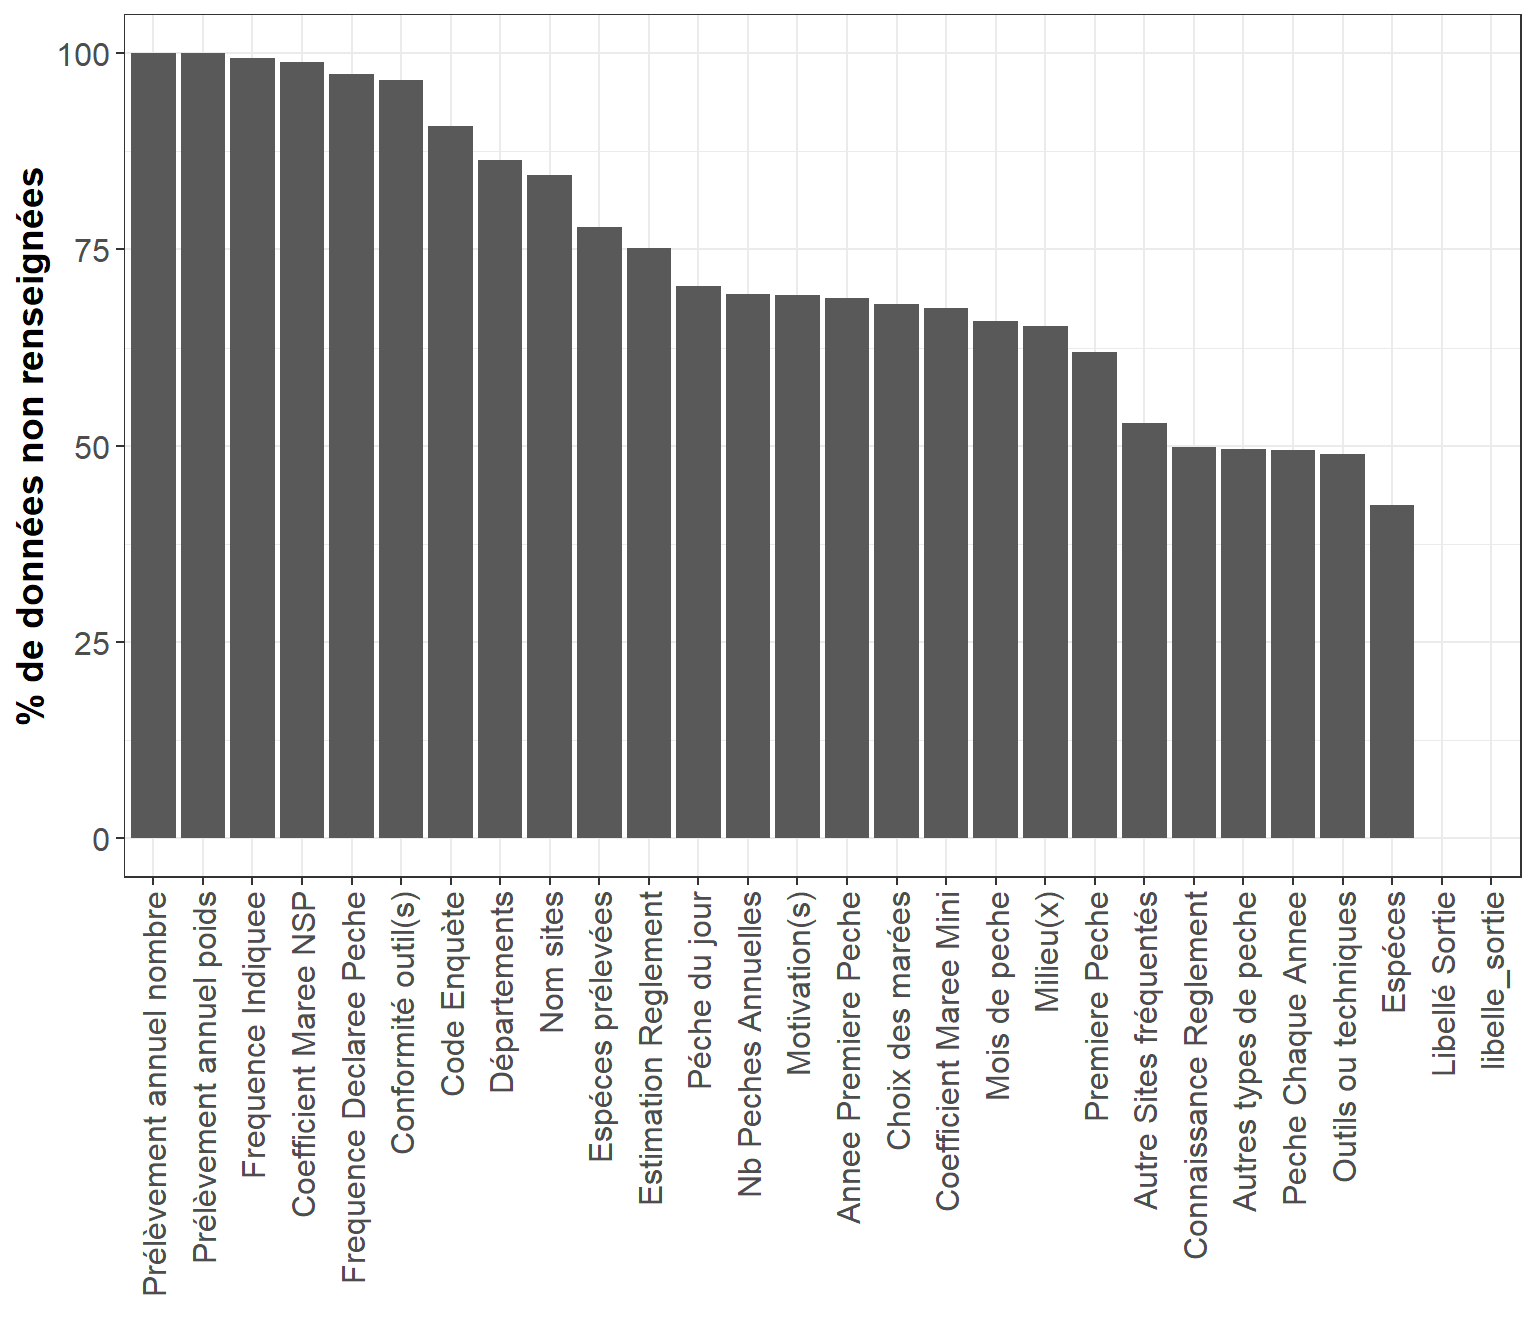
\includegraphics{obade_descriptbaseLifePAP_files/figure-latex/pratPeche.na-1.pdf}

\end{document}
